\documentclass[hyperref, a4paper]{article}

\usepackage{geometry}
\usepackage{marginnote}
\usepackage{float}
\usepackage{titling}
\usepackage{titlesec}
% No longer needed, since we will use enumitem package
% \usepackage{paralist}
\usepackage{enumitem}
\usepackage{footnote}
\usepackage{enumerate}
\usepackage{amsmath, amssymb, amsthm}
\usepackage{mathtools}
\usepackage{bbm}
\usepackage{cite}
\usepackage{graphicx}
\usepackage{subcaption}
\usepackage{physics}
\usepackage{tensor}
\usepackage{siunitx}
\usepackage{booktabs}
\usepackage[version=4]{mhchem}
\usepackage{tikz}
\usepackage{xcolor}
\usepackage{listings}
\usepackage{autobreak}
\usepackage[ruled, vlined, linesnumbered]{algorithm2e}
\usepackage{xr-hyper}
\usepackage[colorlinks,unicode]{hyperref} % , linkcolor=black, anchorcolor=black, citecolor=black, urlcolor=black, filecolor=black
\usepackage{prettyref}

% Page style
\geometry{left=3.18cm,right=3.18cm,top=2.54cm,bottom=2.54cm}
\titlespacing{\paragraph}{0pt}{1pt}{10pt}[20pt]
\setlength{\droptitle}{-5em}
\preauthor{\vspace{-10pt}\begin{center}}
\postauthor{\par\end{center}}

% More compact lists 
% \setlist[itemize]{itemindent=17pt, leftmargin=1pt}

% Math operators
\DeclareMathOperator{\timeorder}{\mathcal{T}}
\DeclareMathOperator{\diag}{diag}
\DeclareMathOperator{\legpoly}{P}
\DeclareMathOperator{\primevalue}{P}
\DeclareMathOperator{\sgn}{sgn}
\newcommand*{\ii}{\mathrm{i}}
\newcommand*{\ee}{\mathrm{e}}
\newcommand*{\const}{\mathrm{const}}
\newcommand*{\suchthat}{\quad \text{s.t.} \quad}
\newcommand*{\argmin}{\arg\min}
\newcommand*{\argmax}{\arg\max}
\newcommand*{\normalorder}[1]{: #1 :}
\newcommand*{\pair}[1]{\langle #1 \rangle}
\newcommand*{\fd}[1]{\mathcal{D} #1}
\DeclareMathOperator{\bigO}{\mathcal{O}}
\DeclareMathOperator{\object}{Ob}
\DeclareMathOperator{\morphism}{Hom}

% TikZ setting
\usetikzlibrary{arrows,shapes,positioning}
\usetikzlibrary{arrows.meta}
\usetikzlibrary{decorations.markings}
\tikzstyle arrowstyle=[scale=1]
\tikzstyle directed=[postaction={decorate,decoration={markings,
    mark=at position .5 with {\arrow[arrowstyle]{stealth}}}}]
\tikzstyle ray=[directed, thick]
\tikzstyle dot=[anchor=base,fill,circle,inner sep=1pt]
\usetikzlibrary{fadings}
\usetikzlibrary{patterns}
\usetikzlibrary{shadows.blur}
\usetikzlibrary{shapes}

% Algorithm setting
% Julia-style code
\SetKwIF{If}{ElseIf}{Else}{if}{}{elseif}{else}{end}
\SetKwFor{For}{for}{}{end}
\SetKwFor{While}{while}{}{end}
\SetKwProg{Function}{function}{}{end}
\SetArgSty{textnormal}

\newcommand*{\concept}[1]{{\textbf{#1}}}

\newrefformat{fig}{Figure~\ref{#1}}

% Embedded codes
\lstset{basicstyle=\ttfamily,
  showstringspaces=false,
  commentstyle=\color{gray},
  keywordstyle=\color{blue}
}

% Disable unsupported commands in bookmark titles 
\pdfstringdefDisableCommands{%
  \def\\{}%
  \def\texttt#1{<#1>}%
  \def\mathbb#1{#1}%
}
\pdfstringdefDisableCommands{\def\eqref#1{(\ref{#1})}}

\makeatletter
\pdfstringdefDisableCommands{\let\HyPsd@CatcodeWarning\@gobble}
\makeatother

\title{Scattering in Relativistic Quantum Field Theories by Prof. Dingyu Shao}
\author{Jinyuan Wu}

\begin{document}

\maketitle

\section{Interaction correlation functions of scalar field}

Suppose the vacuum state $\ket*{\Omega}$ of a field theory with interaction is not orthogonal to the vacuum state $\ket*{0}$ of the free theory.
\marginnote{Peskin Section 4.2}
In order to build connection between the two states, we imaginarily set $\ket*{0}$ to be the initial state and turn on the interaction, 
and make the excited components in $\ket*{0}$ ``relaxed'' back to $\ket*{\Omega}$.
We add an imaginary part to the time to make this happen and we have 
\[
    |\Omega\rangle=\lim _{T \rightarrow \infty(1-\ii \epsilon)}\left(e^{-i E_{0} T}\langle\Omega \mid 0\rangle\right)^{-1} e^{-\ii H T}|0\rangle.
\]
\begin{equation}
    \ket*{\Omega} = \lim_{T \to \infty(1 - \ii \epsilon)} (\ee^{- \ii E_0 (t - (-T))} \braket*{\Omega}{0})^{-1} U(t_0, -T) \ket*{0},
\end{equation}
Suppose $x^0 > y^0 > t_0$, we have 
\[
    \begin{aligned}
        \expval*{\timeorder[\phi(x) \phi(y)]}{\Omega} 
    \end{aligned}
\]

Note that Peskin (4.29) is \emph{not} obtained by simply taking the conjugate transpose of (4.27).
If so, we will see $\lim_{T \to \infty (1 + \ii \epsilon)}$ in (4.29).

In the end we have
\begin{equation}
    \expval*{\timeorder[\phi(x) \phi(y)]}{\Omega} = \lim_{T \to \infty(1 - \ii \epsilon)} \frac{\expval*{\timeorder \phi_\text{I}(x) \phi_\text{I}(y) \exp (- \ii \int_{-T}^T \dd{t} H_\text{I}(t))}{0}}{\expval*{\timeorder \exp(- \ii \int_{-T}^T \dd{t} H_\text{I}(t))}{0}}.
\end{equation}

\section{$S$-matrices of scalar fields}

The correlation function and the $S$-matrix can be related using the LSZ reduction formula. \marginnote{Peskin Section 7.2}
We only need to calculate connected (here the word means every subdiagram is connected to at least one 
external line; It is not necessary to require the whole diagram being connected) and amputated diagrams.

To remove trivial ``nothing happening'' processes, we make the decomposition \marginnote{Peskin (4.72) and (4.73)}
\begin{equation}
    S = \mathbbm{1} + \ii T ,
\end{equation}
and we define 
\begin{equation}
    \ _0\mel{p_1, p_2, \ldots, p_m}{T}{q_1, q_2, \ldots, q_n}_0 = (2\pi)^{m+n} \delta^{(4)}(\sum p - \sum q) \mathcal{M}(p_1, p_2, \ldots, p_m \to q_1, q_2, \ldots, q_n).
\end{equation}

\section{Cross sections}

\begin{figure}
    \centering
    %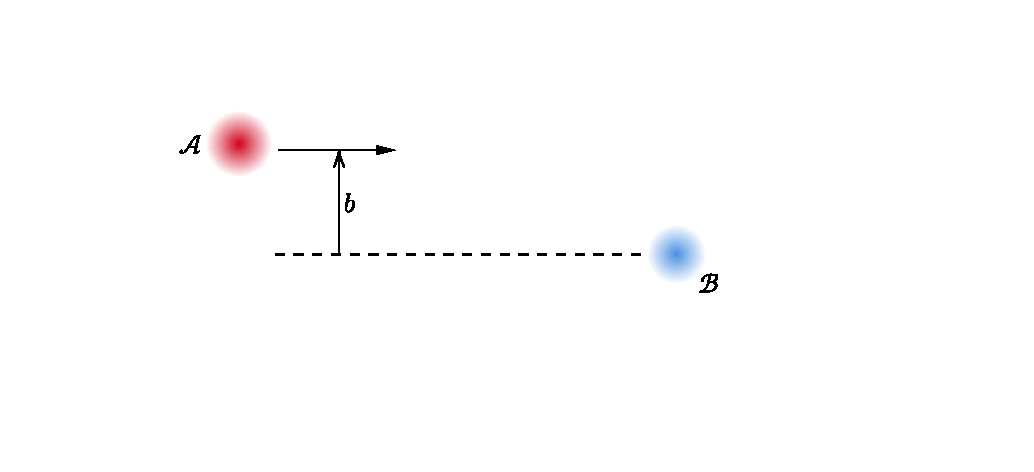
\includegraphics[width=\textwidth]{scattering-parameter.pdf}
    

% Gradient Info
  
\tikzset {_6ptlm6g7t/.code = {\pgfsetadditionalshadetransform{ \pgftransformshift{\pgfpoint{0 bp } { 0 bp }  }  \pgftransformscale{1 }  }}}
\pgfdeclareradialshading{_y5vaxgag9}{\pgfpoint{0bp}{0bp}}{rgb(0bp)=(0.29,0.56,0.89);
rgb(0bp)=(0.29,0.56,0.89);
rgb(0bp)=(0.29,0.56,0.89);
rgb(25bp)=(1,1,1);
rgb(400bp)=(1,1,1)}

% Gradient Info
  
\tikzset {_f8ci9uoe5/.code = {\pgfsetadditionalshadetransform{ \pgftransformshift{\pgfpoint{0 bp } { 0 bp }  }  \pgftransformscale{1 }  }}}
\pgfdeclareradialshading{_jj9izx5r0}{\pgfpoint{0bp}{0bp}}{rgb(0bp)=(0.82,0.01,0.11);
rgb(0bp)=(0.82,0.01,0.11);
rgb(21.33928571428571bp)=(1,1,1);
rgb(400bp)=(1,1,1)}
\tikzset{every picture/.style={line width=0.75pt}} %set default line width to 0.75pt        

\begin{tikzpicture}[x=0.75pt,y=0.75pt,yscale=-1,xscale=1]
%uncomment if require: \path (0,300); %set diagram left start at 0, and has height of 300

%Straight Lines [id:da8003891255178548] 
\draw  [dash pattern={on 4.5pt off 4.5pt}]  (176,162.67) -- (414,162.67) ;
%Shape: Circle [id:dp17109836620556096] 
\draw  [draw opacity=0][shading=_y5vaxgag9,_6ptlm6g7t] (414,162.67) .. controls (414,152.17) and (422.51,143.67) .. (433,143.67) .. controls (443.49,143.67) and (452,152.17) .. (452,162.67) .. controls (452,173.16) and (443.49,181.67) .. (433,181.67) .. controls (422.51,181.67) and (414,173.16) .. (414,162.67) -- cycle ;
%Straight Lines [id:da3766896901237009] 
\draw    (172,96) -- (251,96) ;
\draw [shift={(253,96)}, rotate = 180] [fill={rgb, 255:red, 0; green, 0; blue, 0 }  ][line width=0.08]  [draw opacity=0] (12,-3) -- (0,0) -- (12,3) -- cycle    ;
%Straight Lines [id:da5175887588827652] 
\draw    (217,162.67) -- (217,98) ;
\draw [shift={(217,96)}, rotate = 90] [color={rgb, 255:red, 0; green, 0; blue, 0 }  ][line width=0.75]    (10.93,-3.29) .. controls (6.95,-1.4) and (3.31,-0.3) .. (0,0) .. controls (3.31,0.3) and (6.95,1.4) .. (10.93,3.29)   ;
%Shape: Circle [id:dp7829241030793856] 
\draw  [draw opacity=0][shading=_jj9izx5r0,_f8ci9uoe5] (128,92) .. controls (128,78.19) and (139.19,67) .. (153,67) .. controls (166.81,67) and (178,78.19) .. (178,92) .. controls (178,105.81) and (166.81,117) .. (153,117) .. controls (139.19,117) and (128,105.81) .. (128,92) -- cycle ;

% Text Node
\draw (446,173.07) node [anchor=north west][inner sep=0.75pt]    {$\mathcal{A}$};
% Text Node
\draw (219,129.33) node [anchor=west] [inner sep=0.75pt]    {$\boldsymbol{b}$};
% Text Node
\draw (130,92) node [anchor=east] [inner sep=0.75pt]    {$\mathcal{B}$};


\end{tikzpicture}

    \caption{A typical scattering scenario, where $\vb*{b}$ is the scattering parameter}
    \label{fig:scattering-params}
\end{figure}

A scattering experiment involves a large number of independent processes, each of which is like the following: \marginnote{Peskin 4.5}
\begin{equation}
    k_\mathcal{A} + k_\mathcal{B} \longrightarrow \sum_{i} p_i.
\end{equation}
Since the absolute position is not important, in the (macroscopic) description of the scattering experiment, 
we have the concept of \concept{scattering parameter}, which is depicted in Peskin Figure~4.2 or 
in \prettyref{fig:scattering-params}. We see that the possible values of $\vb*{b}$ form a two-dimensional plane.
Usually, the length scale of the probabilistic distribution of $\vb*{b}$ is much larger than the typical length
scale of particle scattering, and in this way, the scatter experiment can be characterized by the 
\concept{cross section}. Suppose we generate a series of independent scattering events, 
in which $\vb*{v}$'s distribute uniformly in an area of $A$. 
Suppose the number of events is $N(\text{total})$, we have 
\[
    N(\text{total}) = n_\mathcal{B} A, 
\]
where $n_\mathcal{B}$ is the density of incident $\mathcal{B}$ particles on the plane of $\vb*{b}$.
Suppose among the $N(\text{total})$ events, $N(C)$ events of type $C$ occurs, and we have 
\[
    N(C) = \int \dd[2]{\vb*{b}} n_\mathcal{B} \mathcal{P}_C(\vb*{b}).
\]
If the scattering events are merely ``shooting a classical target'', then we just have 
\begin{equation}
    N(C) = \sigma n_\mathcal{B},
    \label{eq:def-cross-section}
\end{equation}
where $\sigma$ is the cross section of the target. We can still calculate the $\sigma$ in 
\eqref{eq:def-cross-section} for other kind of scattering events, and the most general form of $\sigma$ is therefore \marginnote{Peskin (4.75)}
\begin{equation}
    \sigma = \int \dd[2]{\vb*{v}} \mathcal{P}(\vb*{b}).
    \label{eq:cross-section}
\end{equation}
Of course, if there are uncountably types of events, then we have 
\begin{equation}
    \dd{\sigma} = \int \dd[2]{\vb*{v}} \dd\mathcal{P}(\vb*{b}).
    \label{eq:diff-cross-section}
\end{equation}

For a scattering experiment in particle physics, the output states are distributed in the momentum space. 
What can be measured by detectors are just momentum eigenstates, since their resolution of length is rough.
We therefore have \marginnote{Peskin (4.74)}
\begin{equation}
    \dd\mathcal{P}(\mathcal{A B} \rightarrow 12 \ldots n)=\left(\prod_{f} \frac{\dd^{3} \vb*{p}_{f}}{(2 \pi)^{3}} \frac{1}{2 E_{f}}\right) | \prescript{}{\text{out}} \langle {p}_{1} \cdots {p}_{n} \mid \phi_{\mathcal{A}} \phi_{\mathcal{B}}\rangle_{\text {in }}|^{2}.
    \label{eq:peskin-4.74}
\end{equation} 
The significance of the scattering parameter means we cannot consider the input state as momentum eigenstates, 
because if so, the positional uncertainty will be infinity. That is why the input state in \eqref{eq:peskin-4.74} 
is written as a wave packet state, where \marginnote{Peskin (4.68)}
\begin{equation}
    \left|\phi_{\mathcal{A}} \phi_{\mathcal{B}}\right\rangle_{\text {in }}=\int \frac{\dd^{3} \vb*{k}_{\mathcal{A}}}{(2 \pi)^{3}} \int \frac{\dd^{3} \vb*{k}_{\mathcal{B}}}{(2 \pi)^{3}} \frac{\phi_{\mathcal{A}}\left(\vb*{k}_{\mathcal{A}}\right) \phi_{\mathcal{B}}\left(\vb*{k}_{\mathcal{B}}\right) e^{-i \vb*{b} \cdot \vb*{k}_{\mathcal{B}}}}{\sqrt{\left(2 E_{\mathcal{A}}\right)\left(2 E_{\mathcal{B}}\right)}}\left|{k}_{\mathcal{A}} {k}_{\mathcal{B}}\right\rangle_{\text {in }},
\end{equation}
where the $\sqrt{2 E}$ factors are used to guarantee that \marginnote{Peskin (4.66)}
\begin{equation}
    \langle\phi \mid \phi\rangle=1 \quad \text { if } \quad \int \frac{\dd^{3} \vb*{k}}{(2 \pi)^{3}}|\phi(\vb*{k})|^{2}=1.
\end{equation}
Note that here we are using the Lorentz covariant integral measure (see \href{../qft1-homework/1/1.pdf}{here})
in the momentum space. Now we see that according to \eqref{eq:diff-cross-section}, we have Peskin (4.76).

Here we do not repeat the derivation in Peskin from (4.76) to (4.85), but just highlight some subtle details
About the discussion around (4.77). There are $2 \times (3 + 3) = 12$ integral variables in (4.76),
and the $\delta$-function arising from integrating $\vb*{b}$ and the two $\delta$-functions from 
the definition of $\mathcal{M}$ pose in total $2 + 4 + 4 = 10$ constraints. Therefore, we need to 
integrating two variables after these constraints are taken into account. This can also be seen in 
(4.78), where there are six integral variables and a four-dimensional $\delta$-function.

What we want to do is to derive (4.78) from (4.76). Therefore, we need to integrate $\bar{\vb*{k}}_i$
variables. That is why we can see words like ``all six of the $\bar{k}$ integrals in (4.76)''.
Also, it seems the authors use $k^\bot$ to denote $(k_x, k_y)$.

The two $\delta$-functions from $\mathcal{M}$ requires $\sum k_i = \sum \bar{k}_i$, and we know 
$k_\mathcal{B}^\bot = \bar{k}_\mathcal{B}^\bot$, so $k_\mathcal{A}^\bot = \bar{k}_\mathcal{A}^\bot$,
and so do momenta of $\mathcal{B}$. 

Note that the LHS of (4.77) is just a shorthand of 
\[
    \int \dd{\bar{k}^z_\mathcal{A}} \int \dd{\bar{k}^z_\mathcal{B}} 
    \delta(\bar{k}^z_\mathcal{A} + \bar{k}^z_\mathcal{B} - \underbrace{\sum p^z_f}_{k_\mathcal{A} + k_\mathcal{B}}) 
    \delta(\bar{E}_\mathcal{A} + \bar{E}_\mathcal{B} - \underbrace{\sum E_f}_{E_\mathcal{A} + E_\mathcal{B}}) \phi^*_\mathcal{A}(\bar{\vb*{k}}_\mathcal{A}) \phi^*_\mathcal{B}(\bar{\vb*{k}}_\mathcal{B}) .
\]  
After evaluating this integral, $\bar{k}^z_i$ in $\phi_i^*$'s are replaced by the solution of 
\[
    \bar{k}^z_\mathcal{A} + \bar{k}^z_\mathcal{B} - \underbrace{\sum p^z_f}_{k_\mathcal{A} + k_\mathcal{B}} = 0,
    \quad \bar{E}_\mathcal{A} + \bar{E}_\mathcal{B} - \underbrace{\sum E_f}_{E_\mathcal{A} + E_\mathcal{B}},
\]
which is just $\bar{k}^z_i = k^z_i$. That is why in (4.78) we just see $\abs*{\phi_i(\vb*{k}_i)}^2$.

(4.86) is proved in (7.49).

\end{document}